% Autor: Elias Welt
\section{Quiz-Modul (Quiz.jsx \& QuizModal.jsx)}

Das Quiz-Modul bündelt alle Funktionen für interaktives Lernen durch Abfragen. Es besteht aus zwei eng verzahnten Komponenten: \texttt{Quiz.jsx} übernimmt die Übersicht aller vorhandenen Quizzes sowie die vollständige Durchführungslogik, während \texttt{QuizModal.jsx} als Modal für Create- und Update-Operationen dient.

\begin{figure}[h]
    \centering
    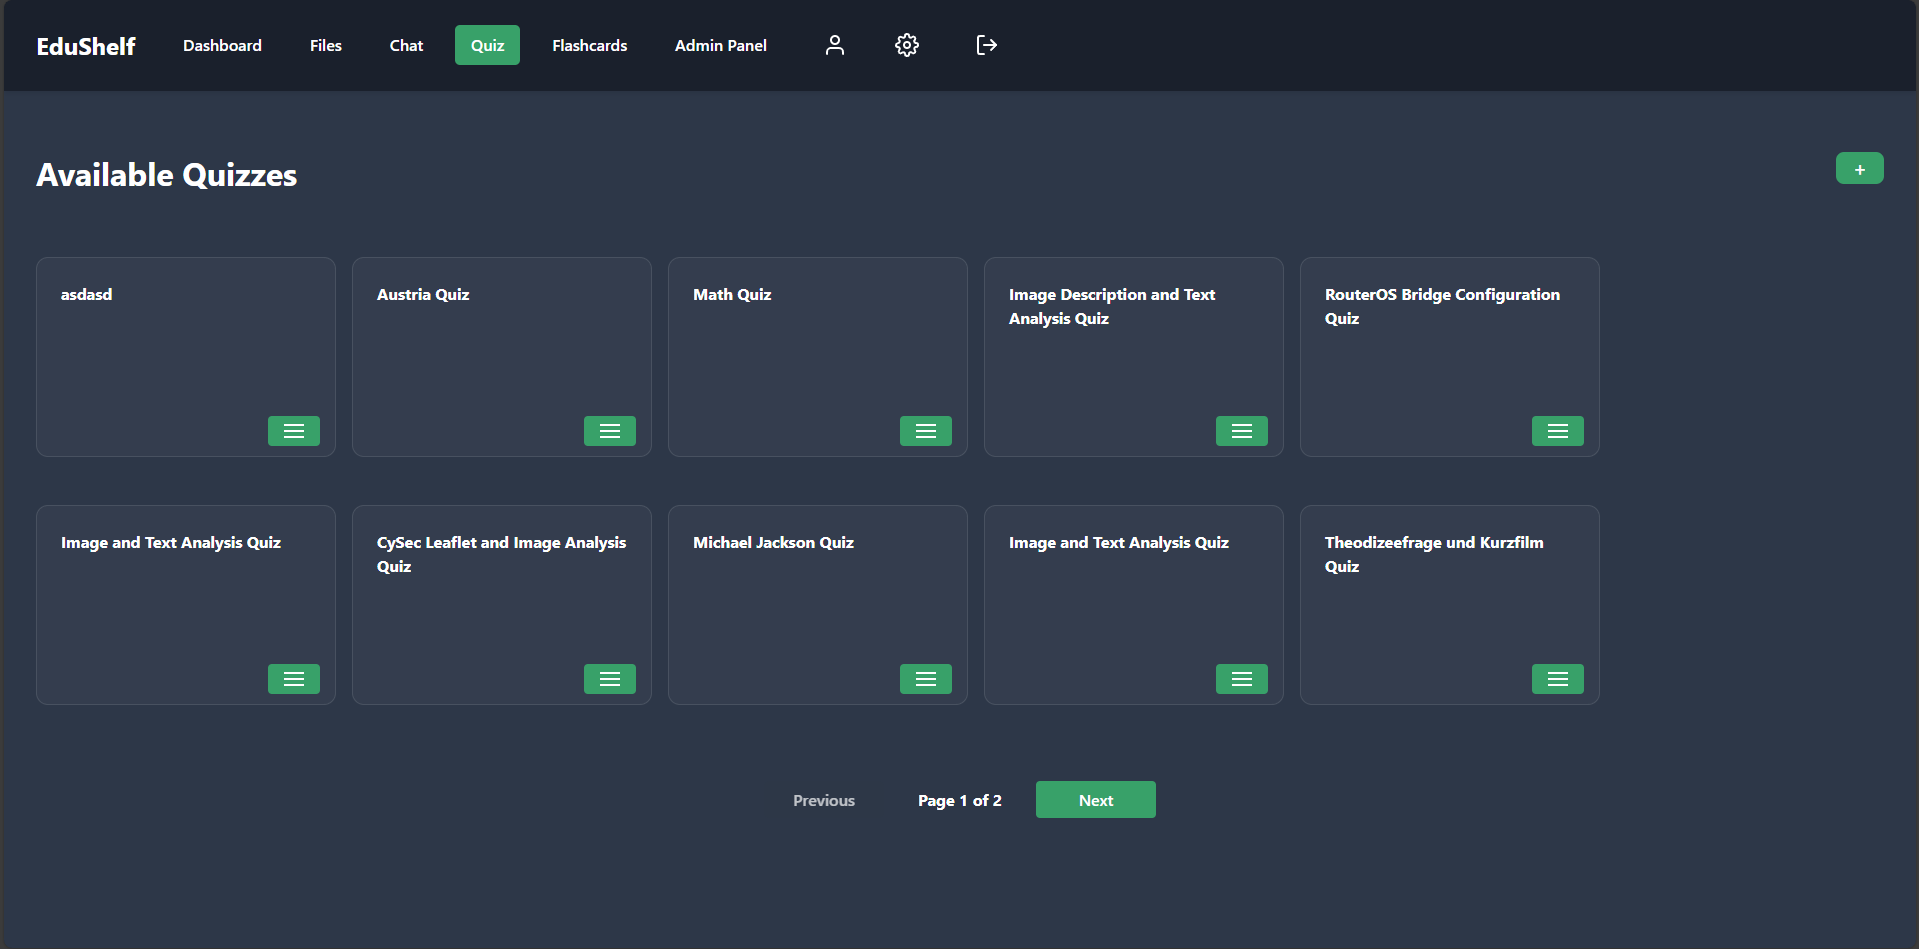
\includegraphics[width=0.92\textwidth]{img/avail-quizzes-dark-mode}
    \caption{Übersicht aller verfügbaren Quizzes im Dark-Mode}
    \label{fig:quiz-overview}
\end{figure}


\subsection{Datenstruktur}

Ein Quiz besteht aus einem Titel und einer Liste von Fragen. Jede Frage enthält wiederum eine Liste von Antworten, wobei eine oder mehrere als korrekt markiert sind. Diese hierarchische Struktur wird im State als verschachteltes Array-Objekt abgebildet:

\begin{lstlisting}[language=JavaScript, caption={Verschachtelte Datenstruktur eines Quiz}]
const [questions, setQuestions] = useState([
  { 
    text: '', 
    answers: [{ text: '', isCorrect: false }] 
  }
]);
\end{lstlisting}

\subsection{Ablauf eines Quiz}

Der Zustand während eines laufenden Quizzes wird durch mehrere State-Variablen gesteuert:
\begin{itemize}
    \item \texttt{currentQuestionIndex}: Index der aktuell angezeigten Frage
    \item \texttt{score}: Anzahl der bisher korrekt beantworteten Fragen
    \item \texttt{selectedAnswerId}: Um eine Mehrfachauswahl zu verhindern und visuelles Feedback zu geben
    \item \texttt{showScore}: Ein Boolean-Flag, das nach der letzten Frage auf \texttt{true} gesetzt wird, um die Ergebnisanzeige zu rendern
\end{itemize}

\begin{figure}[h]
    \centering
    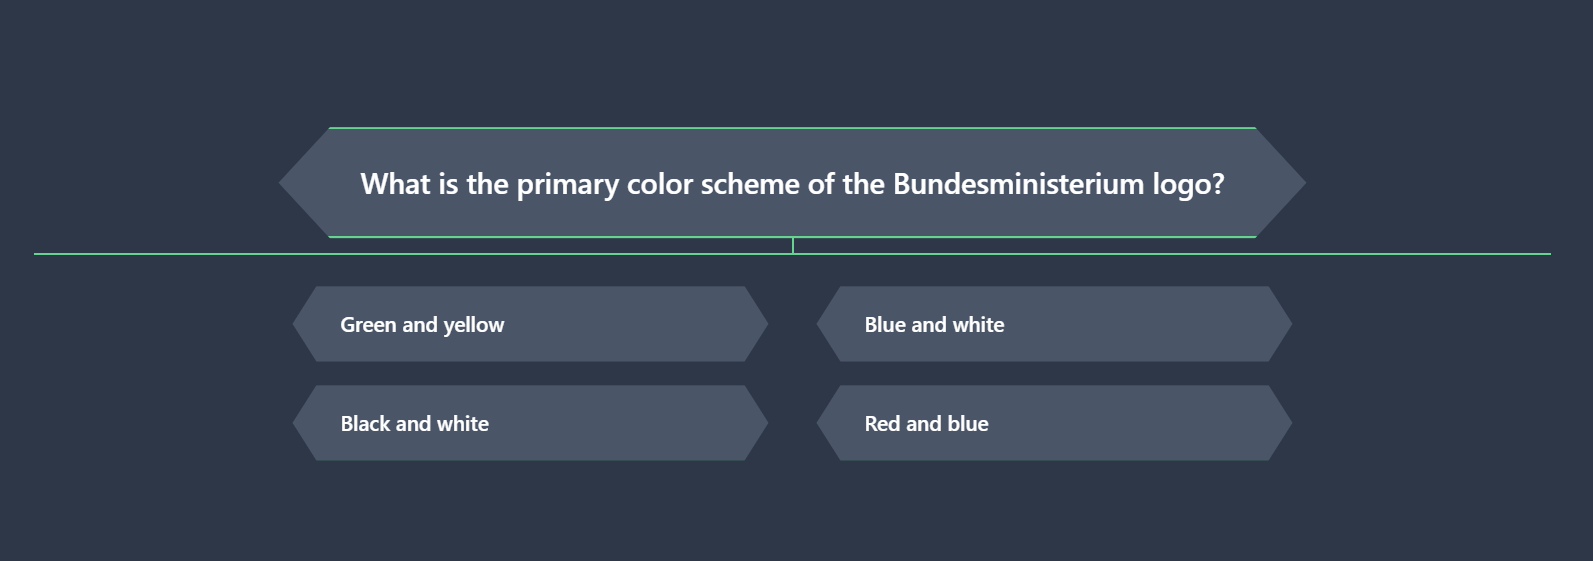
\includegraphics[width=0.92\textwidth]{img/quiz-dark-mode}
    \caption{Quiz-Durchführung mit Antwort-Feedback im Dark-Mode}
    \label{fig:quiz-run}
\end{figure}

Das visuelle Feedback -- Grün für richtig, Rot für falsch -- wird durch CSS-Klassen gesteuert, die dynamisch basierend auf der Korrektheit der Antwort zugewiesen werden. Nach Beantwortung einer Frage wird \texttt{selectedAnswerId} gesetzt und alle Antwort-Buttons werden deaktiviert, um eine Mehrfachauswahl zu verhindern.


\subsection{Quiz-Editor (QuizModal.jsx)}

Die Erstellung und Bearbeitung von Quizzes erfolgt über \texttt{QuizModal.jsx}. Der Editor ermöglicht dynamisch das Hinzufügen und Entfernen von Fragen und Antworten.

\begin{figure}[h]
    \centering
    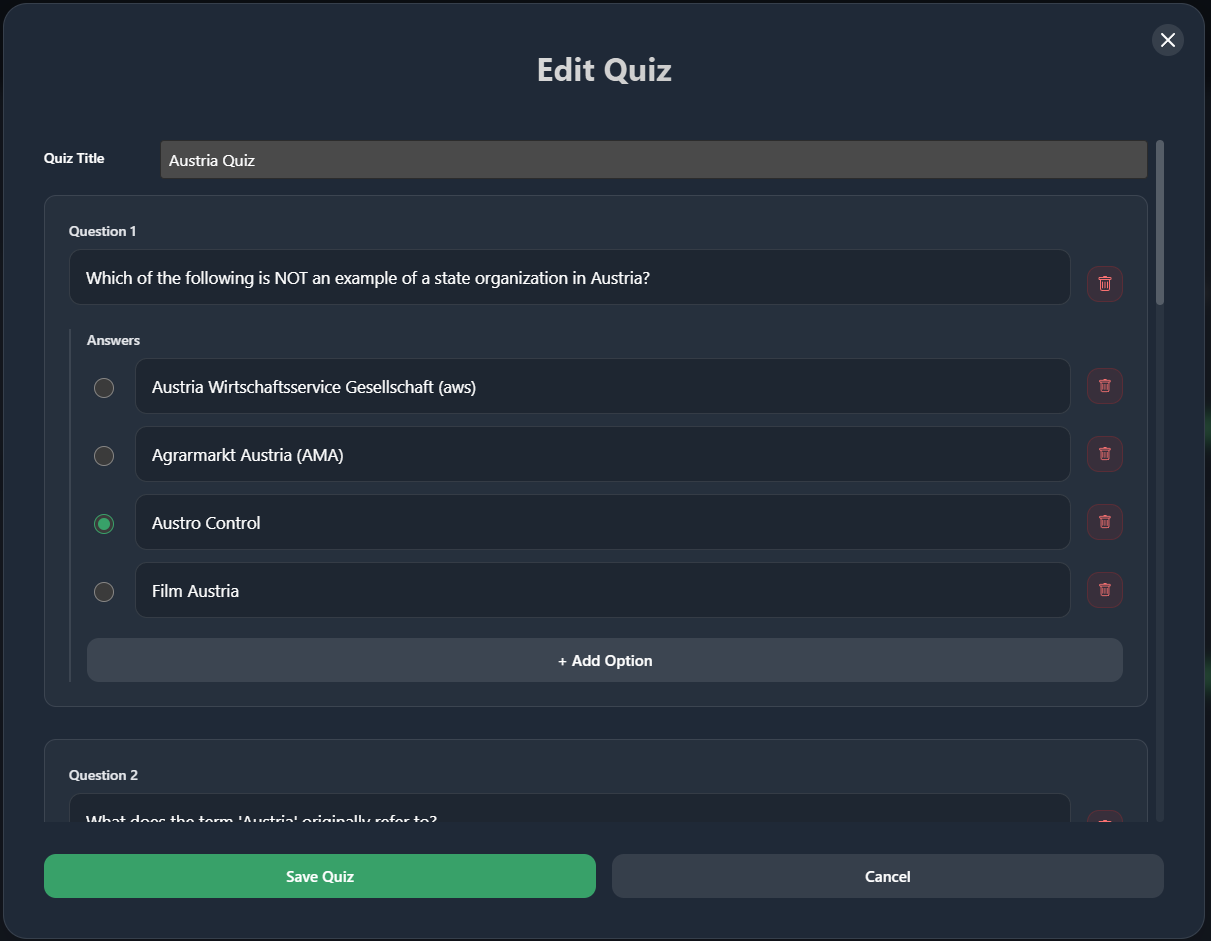
\includegraphics[width=0.75\textwidth]{img/edit-quiz-darkmode}
    \caption{Quiz-Editor zum Erstellen und Bearbeiten von Quizzes}
    \label{fig:quiz-edit}
\end{figure}

\subsubsection{Dynamische Formular-Manipulation}

Beim Ändern eines Antworttextes darf der State nicht direkt mutiert werden. Stattdessen muss eine Kopie der betroffenen Ebenen erstellt werden -- das Prinzip der Immutability in React:

\begin{lstlisting}[language=JavaScript, caption={Update-Logik für verschachtelte Antworten}]
const handleAnswerChange = (questionIndex, answerIndex, event) => {
    const newQuestions = [...questions]; // Kopie des Arrays
    newQuestions[questionIndex].answers[answerIndex].text 
        = event.target.value;
    setQuestions(newQuestions); // Re-Render ausloesen
};
\end{lstlisting}

Beim Speichern (\texttt{handleSubmit}) wird unterschieden, ob ein neues Quiz erstellt (\texttt{POST}) oder ein bestehendes bearbeitet (\texttt{PUT}) wird. Nach erfolgreicher API-Antwort ruft das Modal den übergebenen Callback \texttt{onQuizSaved()} auf, damit die Elternkomponente ihre Liste ohne erneuten Fetch aktualisiert.

